\documentclass[pdftex,10pt]{article}
\usepackage{fullpage}
\usepackage{graphicx}
\usepackage{natbib}
\usepackage{amsmath}

\title{Storm Surges}

\date{\today}

\begin{document}
\maketitle

\begin{abstract}
Abstract to be completed
\end{abstract}

\section{Introduction}\label{sec:intro}


%some general intro paragraph here

%my attempt at physical oceanopgraphy SoG- Susan feel free to edit.
The Strait of Georgia is a strongly stratified, semi-enclosed body of water located between Vancouver Island and the mainland of British Columbia. It is part of a larger system of waterways collectively known as the Salish Sea and is connected to the Pacific Ocean via the Strait of Juan de Fuca and Johnstone Strait. Several features related to the physical oceanopgraphy of this region render it a challenge to model numerically. The outflow from the Fraser River in the late spring is the primary source fresh water within the Strait of Georgia and leads to large vertical density gradients in the summer months. Additionally, strong tidal mixing through the San Juan and Gulf Islands produces horizontal density gradients that separate the saline waters of the Strait of Juan de Fuca and the fresher water of the Strait of Georgia. It is important to accurately represent the vertical mixing in this region as it sets the rate of export of fresh water through estuarine circulation. The strong and fast tidal currents through the narrow channels of the north, such as Discovery Passage and Johnstone Strait, pose a particular challenge for numerical models. Yet, several modelling efforts for this region exist, ranging in choices of grid structure, mixing parametrizations, and domain size and extent. 

%overview oF SoG/Salish Sea models


%intro to storm surges
Many coastal communities in the Strait of Georgia are at risk to flooding and property damaged caused by storm surges, a natural hazard arising from the combination of a strong wind storm and high tide. The low atmospheric pressure associated with a storm acts as an inverse barometer elevating the sea level. This effect in combination with strong winds pushing water up against the coast can cause flooding, particularly if the storm occurs during an unusually high tide.  Additionally, there is a small contribution to increased sea level due to the thermal expansion of water during warmer years set by the El Nino Southern Oscillation (ENSO) \citep{abeys2011extreme}. %more on past events, significance

Communities in the Strait of Georgia are partiuclarly susceptible to storm surges in the winter months when there is an increased propensity for storms and south easterly winds and geostrophic adjustment lead to higher coastal waters \citep{danard2003storm}. In the summer months, the wind direction changes to north westerly and mean sea level is lower. 
%work on this

%storm surge modelling

%overview of paper: model configuration, model evaluation, storm surge hindcasts.
This paper is organized as follows: an overivew of the model configuration and domain including a description of open and surface boundary conditions is provided in section \ref{sec:config}. This section also describes the ocean model we have employed as well as choices in grid structure and mixing parameterizations. Next, section \ref{sec:model} presents an evaluation of model performance through comparisons of tidal amplitudes and phases with observations. The model's accuracy in producing storm surge hindcasts is also assesed in section \ref{sec:storm}. Finally, a summary and discussion of future research goals is provided in section \ref{sec:diss}.  

\section{Model Configuration}\label{sec:config}
%To be included: NEMO overview, tides, rivers, bathymetry, atmospheric forcing, vertical/lateral mixing, boundary conditions, grid. 

%A section about how we configured the model for SoG 
We have used the Nucleus for European Modelling of the Ocean (NEMO) framework in its regional configuration to develop an ocean model for the Strait of Georgia and Salish Sea. NEMO is a highly modularized tool used for studying ocean physics, ocean-ice interactions, and the biogeochemical properties of the ocean. NEMO's ocean core solves the three-dimensional hydrostatic equations of motion for an incompressible fluid under the Boussinesq approximation on a structured computational grid. Although not used in the present work, NEMO's options for grid nesting and biogeochemical coupling make it a useful tool for studying the complex physics and biogeochemical interactions within the Strait of Georgia. This work focuses on validating the physical set up of the Salish Sea model, in particular, determining appropriate forcing and boundary conditions for accurate reproduction of tidal amplitudes and phases as well as storm surge elevations. Future work will include biogeochemical coupling and data assimilation. 

\subsection{Model domain}
The modelled domain extends from the Strait of Juan de Fuca to Puget Sound to Johnstone Strait as shown in Figure \ref{fig:domain}. Bathymetry from the Cascadia physiography dataset \citep{haugerud1999digital} was smoothed to limit the difference in depth across grid cells. For model stability, additional smoothing at the Strait of Juan de Fuca western boundary was imposed to achieve constant depth across the first ten grid cells. As depicted in Figure \ref{fig:domain}, the numerical grid is rotated $29^{\circ}$ counter-clockwise of North in order to maintain computational efficiency since currents within the Strait of Georgia are mainly aligned with this rotated axis. 

The curvilinear orthogonal numerical grid has been divided into 398 by 898 by 40 grid cells, which results in an almost uniform horizontal resolution with grid spacing approximately 440 m by 500 m. The 40 vertical $z$-levels were stretched gradually in order to achieve higher resolution in the surface layer, with 1 m vertical grid spacing down to about 10 m in depth. Below 10m the grid was stretched to a maximum grid spacing of 27 m at the lowest layer. At the bottom boundary, partial $z$-levels were utilized in order to limit large changes in bathymetry across grid cells \citep{madec2012nemo}. 

In addition to the equations of motion, a prognostic equation for the sea surface height is solved at each time step. The inclusion of the sea surface height equation requires a fairly restrictive time step due to the presence of high speed surface gravity waves. As such, the split-explicit time stepping algorithm is employed, where the free surface and barotropic equations are solved with a smaller time step than that used for the other variables. The model time step is and barotropic time step are 10 s and 2 s respectively. Small vertical grid spacing and large vertical velocities in the Boundary Pass and Haro Strait region impose a fairly restricitive step through the vertical CFL condition.


\begin{figure}[h]
\centering
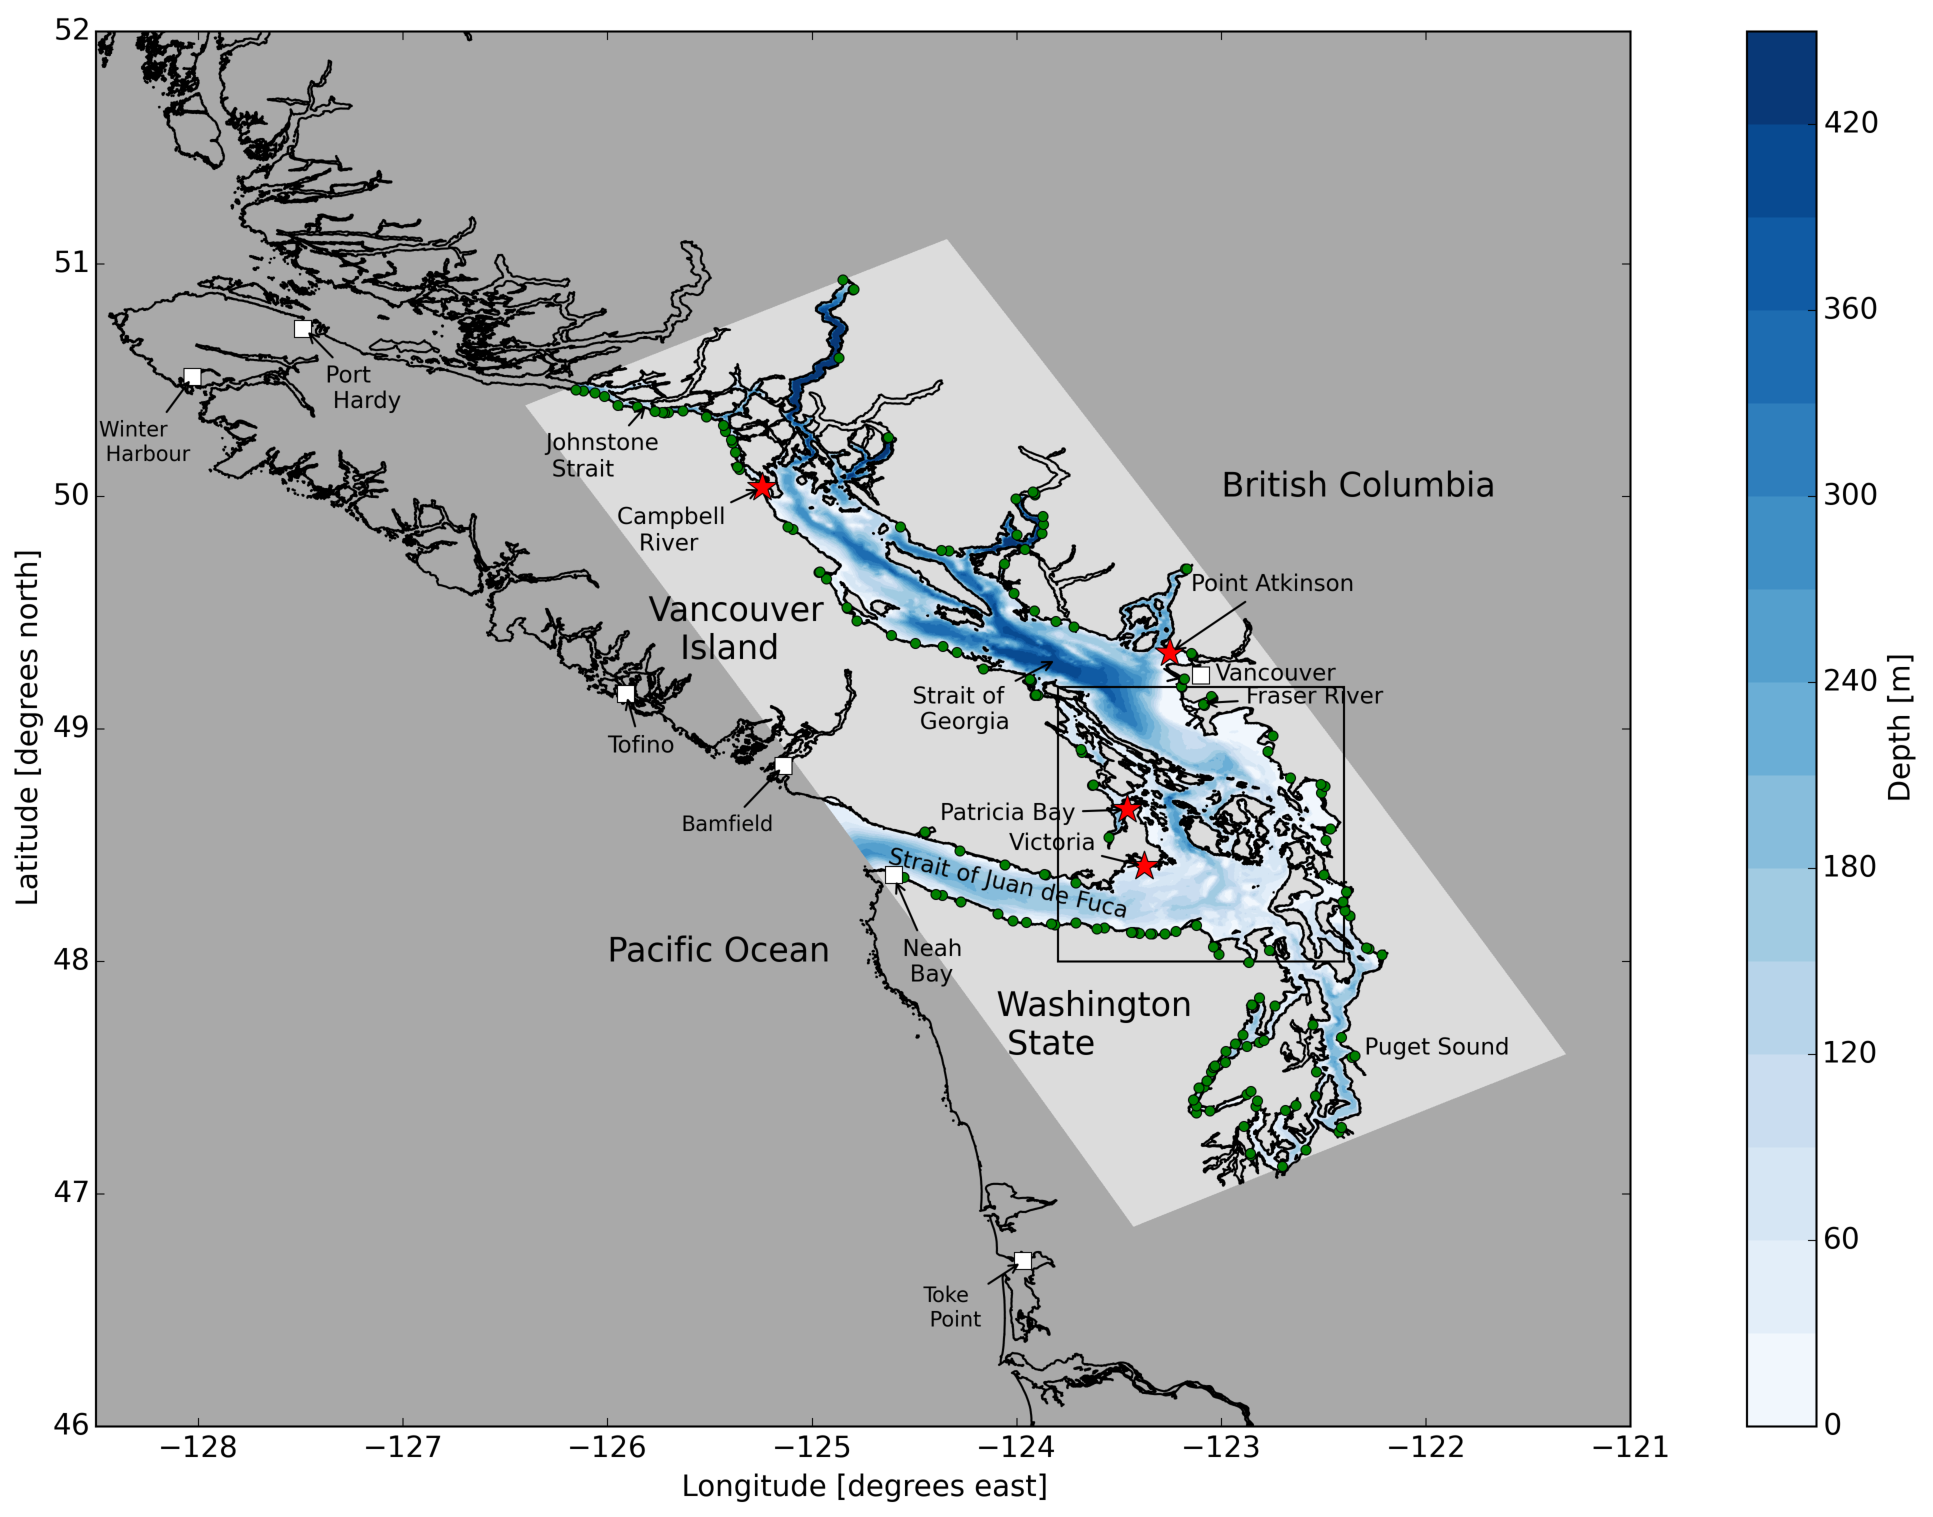
\includegraphics[scale=0.5]{Figures/bathy.pdf}
\caption{Model domain (highlighted area) including bathymetry, rivers (blue circles), and storm surge locations of interest  (red stars).}\label{fig:domain}
\end{figure}
%image needs some work: labels for tide comparisons?

\subsection{Boundary conditions and sub-grid scale processes}
The model includes two open boundaries that connect to the Pacific Ocean, the western boundary of the Strait of Juan de Fuca as well as Johnstone Strait at the north, both of which are forced with eight tidal constituents (K$_1$ ,O$_1$, P$_1$, Q$_1$, M$_2$, K$_2$, N$_2$, S$_2$), temperature and salinity climatologies, and the sea surface height anomaly. Tidal heights and currents at grid points along the Juan de Fuca boundary were extracted from Webtide, an online web prediction model for the northeast Pacific Ocean, which is based on work by \citet{foreman2000webtide}. The Johnstone Strait boundary was forced with current and elevation tidal harmonics measured and calculated by \citet{thomson1980johnstone} for the major M$_2$ and K$_1$ constituents. Additionally, O$_1$ and S$_2$ elevation harmonics from their measurements were employed. The remaining constituents were extrapolated from Webtide. 
% Needs editing! Update when we are finished with tides.

Temperature and salinity at the Juan de Fuca boundary were taken from a weekly climatology which was created from results from a model covering the Salish Sea and the west coast of Vancouver Island \citep{massonfine2012}.  Their results, originally on s-levels were interpolated onto z-levels and then onto the NEMO horizontal grid.  To prepare the climatology all years (1995-2008) were averaged and results, approximately every 15 days, were interpolated to a weekly climatology. The model is relaxed to the forced temperature and salinity over the 10 grid points (about 5km) closest to the open boundaries, using a flow relaxation scheme \citep{engedahl1995use}. %other references?

Sea surface height at the mouth of Juan de Fuca was set using values from the Tofino tide gauge.  A monthly climatology was produced using daily averages from 2000-2010, binning them by month, averaging and setting the yearly mean to zero.  For the storm surge simulations, hourly variations in sea surface height were used.  These values are the Tofino tide gauge values, de-tided and with the zero reset as for the climatology. The storm surge simulations also used the sea surface height anomaly from Port Hardy, forced at the northern boundary in Johnstone Strait. The tidal forcing and sea surface height was used in the barotropic velocity forcing which used the NEMO Flather scheme \citep{flather1994storm, madec2012nemo}.
The baroclinic velocities at the boundary were set to be equal to the values inside the boundary (zero-gradient boundary conditions).  This scheme is not part of core NEMO.  Zero gradient conditions were chosen because the baroclinic velocity at the mouth of Juan de Fuca is primarily estuarine and thus set by density variations between inside and outside the domain.

At coastal boundaries, the partial slip boundary condition, an approximation to no slip, is used. Partial slip allows one to include the frictional effects of lateral boundaries without the restrictive resolution required to represent the lateral boundary layer under no slip conditions. A lateral eddy viscosity of 20 m $^2$ s $^{-1}$ parametrizes horizontal friction and a lateral eddy diffusivity of 20.5 m $^2$ s $^{-1}$ is used.  Bottom friction is represented by a quadratic law for the bottom momentum flux with drag coefficient $C_D = 5\times 10^{-3}$. Vertical turbulence and mixing is calculated through the $k-\epsilon$ configuration of the generic length scale (GLS) turbulence closure \citep{umlauf2003generic} with background vertical eddy viscosity and diffusivity set to $1\times10^{-4}$ and $1\times10^{-5}$ m$^2$ s$^{-1}$ respectively. Details on the NEMO implementation of the partial slip lateral boundary condition, quadratic bottom friction law, and GLS turbulence closure scheme are provided by \citet{madec2012nemo}.

At the ocean surface, meteorological conditions and fresh water input from rivers are included. The ocean surface is forced with momentum and heat fluxes from a 33-km global atmospheric reforcasting model suitable for use in ocean modelling \citep{smith2013new}. Forecasts from the period of 2002-2011 are available. Additionally, the inverse barometric effect of the atmospheric pressure is included, an important consideration in storm surge modelling. 

River input provides a significant volume of freshwater to the Salish Sea and can influence stratification, circulation and primary productivity. However, most rivers in the domain are not gauged so parameterizations were required to represent river flow. \citet{morrison2011rivers} provides a method for estimating freshwater runoff in the Salish Sea region based on precipitation. Monthly runoff volumes for each watershed for each year from 1970 to 2012 were acquired from \citet{morrison2011rivers}, as well as monthly averages. 

Freshwater runoff from each watershed was divided between the rivers in that watershed. The area drained by each river was estimated from Toporama maps by the Atlas of Canada and watershed maps available on the Washington State government website. The watersheds included in our model were Fraser (which represents approximately 44\% of the freshwater input into our domain), Skagit (12\%), East Vancouver Island (North and South) (12\%), Howe (7\%), Bute (7\%), Puget (6\%), Juan de Fuca (5\%), Jervis (4\%) and Toba (3\%). 

The monthly flow from each river was input as a point source in the three grid points closest to the surface at the model point closest to the mouth of each river. Incoming water was assumed to be fresh and at surface temperature. A total of 150 rivers were parameterised by this method and their locations are indicated by the blue dots in Figure \ref{fig:domain}.


Initial conditions for temperature and salinity were taken from a CTD cast in the middle Strait of Georgia taken in Sept 2002 \citep{pawlowiczetal2007}.  Conditions were initially uniform horizontally and velocity was initialized at zero. The model was spun up for a 15.5 months from the initial conditions above, starting Sep 16, 2002, using atmospheric forcing from 2002-2003, climatological temperature and salinity and sea surface height at the boundaries, with tides and climatological river output.  All storm surge runs were started three days prior to the event of interest with zero initial velocities and sea surface height and a stratification profile from model spin up. The modelled sea surface height adjusted to forcing in less than one day. 

\section{Model Evaluation}\label{sec:model}

\subsection{Tidal evaluation}
The model was initially evaluated qualitatively by comparing patterns of tidal amplitude and phase to results from \citep{foreman1995tidal}. For example, the amphidromic dome around Victoria was produced in the M$_2$ results, as well as the monotonic increase in $K_1$ amplitude moving northwards along the Strait of Georgia. Initially, the Johnstone Strait boundary was closed, but modelled M$_2$ amplitudes were too small compared to measured amplitudes... TBC

%perhaps a nice contour map of M2 and K1 amps and phases goes here?

Once our model was reproducing observed tidal patterns, model results were quantitatively evaluated by comparing modelled harmonic constituents to measured harmonic constituents at tidal measuring stations throughout the domain. Comparisons were made using the complex difference ($D$), defined by \citep{foreman1995tidal} as:

\begin{equation}
D = [(A_0 \cos g_0 - A_m \cos g_m)^2 + (A_0 \sin g_0 - A_m \sin g_m)^2]^{1/2}
\end{equation}\label{eq:compdiff}
where $A_0$, $A_m$, $g_0$ and $g_m$ are observed and modelled amplitudes and phases.

%perhaps a table of complex differences at tidal stations similar to Table 1 of Foreman et al (1995)  (such as the one produced by tidetools.calc_diffs_meas_mod) here?
%(would be cool to include the complex differences calculated at the VENUS nodes too)

\begin{table}[h]
\centering 
\begin{tabular}{l l c c c c c c} 
\hline 
& & \multicolumn{3}{c}{M$_2$} & \multicolumn{3}{c}{K$_1$} \\ 
\hline 
Station number & Station name & $R$ & $ \Delta \phi$ (deg) & $D$ (cm) & $R$ & $ \Delta \phi$ (deg) & $D$ (cm) \\
\hline 
               &              &     &                      &          &     &                      &          \\
\hline   
Mean Error     &              &     &                      &          &     &                      &          \\
RMS Error      &              &     &                      &          &     &                      &          \\
\hline  
\end{tabular}
\caption{Comparisons of modelled and observed amplitudes and phases. $R$ is the ratio of modelled to observed amplitude. $\Delta \phi$ is the difference between modelled and observed phase. $D$ is the complex difference. }
\label{tab:comparison} 
\end{table}
%May have to include station numbers and locations on a map? Maybe on the contour map, overlay with stations and green/red dots (hopefully mostly green)
%Should we use the new method of calculating tides?

Complex differences were less than ??cm at all stations in our domain, which was assumed to be acceptable for our purposes. 
%if it's favourable, we could compare our complex differences to Foreman et al (1995), who got an average of D=3cm for M2 and D=2.5cm for K1

\subsection{Stratification} 
%outline: thalweg, plots of winter/summer stratty
%Maybe not this

\section{Storm Surge Hindcasts}\label{sec:storm}
%outline: 
%1. factors contributing to storm surge with focus on Feb 2006 event
%2. Strong wind event but no surge (maybe Dec 2006 or Nov 2009)
%3. High resolution wind (hopefully Dec 2012)
A series of storm surge hindcasts is presented next. Storm surge simulations were started from rest at least three days prior to the event of interest to allow for adjustment of model currents. Stratification conditions from model spin-up at a time close to the event (within 5 days) were chosen to initialize the temperature and salinity fields. Boundary conditions include atmospheric forcing and fresh water input from rivers at the surface, sea surface height anomaly from observations at the open boundary, and tidal forcing with eight tidal constituents. Forcing the model with only eight tidal constituents leads to an error in modelled sea surface height predictions due to the omission of the next leading order tidal constituents such as J$_1$. Comparisons between full tidal predictions and tidal predictions using eight constituents suggest that this error can be up to 40 cm (check) during times of high tidal range, and in particular, during the storm surge season Nov-Feb. As such, storm surge model predictions were corrected by accounting for this error. Additionally, since the sea surface height is calculated about a zero reverence level, the modelled water level is determined by adding a long term average of mean sea level at the specified location to the modelled sea surface height and removing a background anomaly caused by topographic pressure gradients since the atmospheric reforecasting model uses a terrain following coordinate system. (Nancy: I think we need a better way of adjusting come publication time).

Model results have been compared with observations by calculating both the total modelled water level and the modelled residual. The modelled residual is calculated as the difference in model output between a simulation with all forcing conditions and a simulation forced only with tides and rivers. The observed water level is taken from observations by Fisheries and Oceans Canada (citation) and the observed residual is the observations minus tidal predictions. Tidal predictions are calculated using t\_tide \citep{pawlowicz2002classical}, a MATLAB tool that calculates tidal harmonics from a given time series, in this cae, from the year prior surge event on interest. Additionally, several simulations with varying forcing conditions such as removing atmospsheric forcing or removing the sea surface height anomaly at the open boundaries have been completed. 

Several significiant surge or wind events have been considered in detail, as well as an array of hindcasts to asses model ability in a statistical measure. These cases have been used to asses the model's skill in reproducing water level height and surge amplitude and timing during storm events. In addition, the contribution to the surge of several forcing conditions, such as atmospheric forcing and open boundary forcing, has been assessed. We have also examined the spatial variabilty of the surge as it propagates through the domain and have considered a case with high-resolution atmospheric forcing. 

%First, a study of a large surge event on Feb 4, 2006 is presented. This event caused siginificant damage and flooding in Boundary Bay, a community south of Richmond, (citation) and has been chosen as a case study to demonstrate the model's skill in reproducing a storm surge and to quantitatively assess forcing conditions that are important in storm surge hindcasting. Second, an extreme wind event on Dec 15, 2006 is examined. This event produced winds over (x) (citation) but did not result in significant flooding because the storm did not occur at high tide, however, it did result in siginificant property damage due to high winds and waves. This event has been used to understand the spatial and temporal variability of the surge propagation. Next, a large wind event on Nov 18, 2009 that did not result in a siginificant surge or flooding is presented. This case was choosen to identify the model's capability in handling large wind events that do not result in high water levels. Next, a case with high resolution atmospheric forcing for a recent surge on Dec 17, 2012 is discussed. Lastly, these cases presented in detail will be combined with $x$ additional runs for statistical evaluation of model performance. 


\subsection{Factors Contributing to Storm Surges: Feb 4, 2006}

On Feb 4, 2006, a strong storm system with winds over 75 km/hr coinciding with an unsually high tide led to siginificant flooding in coastal comminuties of the Strait of Georgia \citep{romanowski2010storm}. The maximum water level observed at Point Atkinson on this day was 5.49 m, which is 0.8 m higher than the predicted tides, highlighting the significance of this event as it resulted in a large anomaly and also reached water levels close to the highest level ever recorded (5.61 m). A set of simulations from Feb 1 to 8, 2006 under varying forcing conditions has been completed in order to determine the siginicance of each factor contributing to the surge.

The model's ability to reproduce this event is demonstrated in Figure \ref{fig:feb2006} which compares observations and corrected model output at Point Atkinson, Victoria, Patricia Bay, and Campbell River. The timing of maximum water level matches well between the observations and the model at all four locations, the most siginificant contribution to high water level being from the tides. There is also a good match in amplitude of the water level maximum at Point Atkinson and Campbell River, with a relative error less than 4\%. There is only a 7.2 cm difference between observed and modelled water level elevation at Point Atkinson and a 20.9 cm difference at Campbell River. Tthe error at Victoria and Patricia Bay is slightly more siginificant, reaching 9.6\% and 6.3\% respectively (close to 30 cm in each case), partly due to error in tidal amplitudes as discussed above. The precise location and magnitude of the M$_2$ amphidrome around Victoria is very sensitive to model parameters such as bottom friction. 

The error in modelled residuals is also apparent in the panels on the right, most noticeable is an underestimate in maximum residual (or surge) at all locations. There is also a 2-3 hour delay in the timing of the maximum residual except at Victoria where the maximum residual in sync with observations. The errors in maximum residual range from 8.0 cm at Victoria to 28 cm at Campbell River. It is also apparent that Point Atkinson and Campbell River experienced the largest observed surges at 82 cm and 95 cm respectively. The surges at Victoria and Patricia Bay were observed to be 66 cm and 74 cm. 
%Question: is it better to present relative errors or just difference?


\begin{figure}
\centering
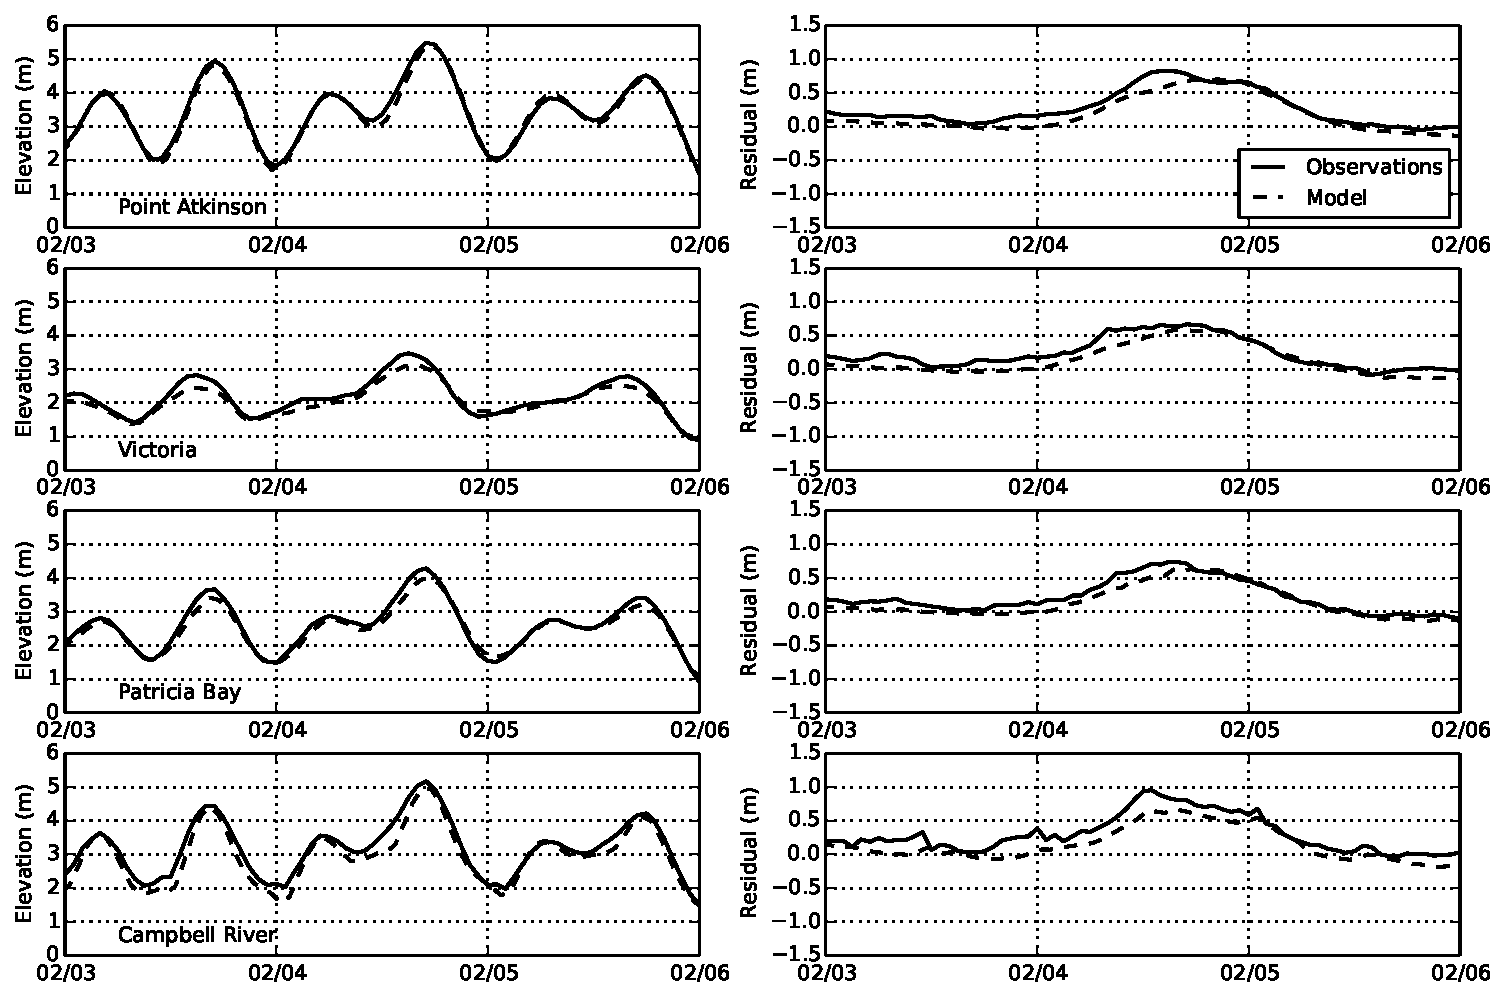
\includegraphics[scale=0.6]{Figures/feb2006_bg.pdf}
\caption{Comparison of observations and model output for the Feb 4, 2006 storm surge. Left: total water level observation (solid) and corrected model (dashed). Right: observed residuals (solid) and modelled residuals (dashed).}
\label{fig:feb2006}
\end{figure}

Next, an assessment of the factors that are most important in scenarios leading up to storm surges is presented in Figure \ref{fig:factors}. The modelled residual from three simulations have been plotted. First, a simulation with all the forcing conditions, including tides, atmospheric forcing, rivers, and sea surface height anomaly, is shown in blue. Additionally, a simulation with all forcing except the atmospheric forcing is presented in green and a simulation with all forcing except the sea surface height anomaly is shown in red. It is clear that the sea surface height anomaly contributes most significantly to the surge at each of these locations. When the sea surface height anomaly is not included as a forcing condition, the surge drops from 70 cm to 15.6 cm at Point Atkinson and its maximum occurs eight hours later.  A similar drop in the maximum surge and delay in timing of the maximum surge is observed at the other locations. The atmospheric model indicates southeasterly winds during the onset of the surge but after the peak surge has passed, the winds shift to westerly. A strong westerly wind would cause an elevated sea surface height at Point Atkinson as water piles against the coast, explaining the delay in peak surge when only atmospheric forcing is used since the winds to shift westerly after the peak surge has passed. A simulation with only wind forcing (no inverse barometer effect or anomaly at open boundary) produces a surge of 9.0 cm at Point Atkinson, a small fraction of the total observed surge. However, this wind-induced surge occurs well after the peak surge from observations and simulations with full forcing.

The contribution to the surge due to atmospheric forcing appears to be geographically dependent, its removal leading to a drop of about 5 cm in the maximum surge at Point Atkinson and 10 cm at Campbell River. When atmospheric forces are neglected the timing of the maximum surge is earlier at Point Atkinson but later at Campbell River. Campbell River exhibits a strong response to atmopsheric conditions during midday on Feb 4, as demonstrated in a two sharp spikes in both the blue and red curves arounf 12:00 hr The green curve, which does not include any atmopsheric focring, does not exhibit this behaviour. The result is a peak surge earlier than in day than the no atmospheric forcing case. This response is also noted in the observations at Campbell River in Figure \ref{fig:feb2006} where the maxmium surge occurs earlier than at the other locations. At Victoria and Patricia Bay, the surge amplitude is mainly unaffected by the atmospheric forcing. 
%maybe look at winds/pressure to see why Vic/Pat Bay aren't affected?. Plan: map of wind vectors from CGRF (not for paper, just for me in aiding with explanation)


These comparisons point to the importance of including, as a forcing condition at the open bounday, the surge entering the domain from the Pacific Ocean. Storms travelling over the Pacific Ocean torwads the west coast of the northern United States and Canada can induce elevated sea levels along the coastline which then enter the Salish Sea sytem through the Strait of Juan de Fuca. In a model domain that does not inlcude the Pacific Ocean, this effect must be inlcuded as a boundary condition. Previous simulations by \citet{murty1995storm} suggest that the inverese barometer effect and the surge entering the system through the Strait of Juan de Fuca contribute most significantly to storm surges in this domain.  A detailed assessment of the effect of the local atmospheric condtions and winds is included later where simulations have been performed with high resolution atmospheric forcing data.  

\begin{figure}
\centering
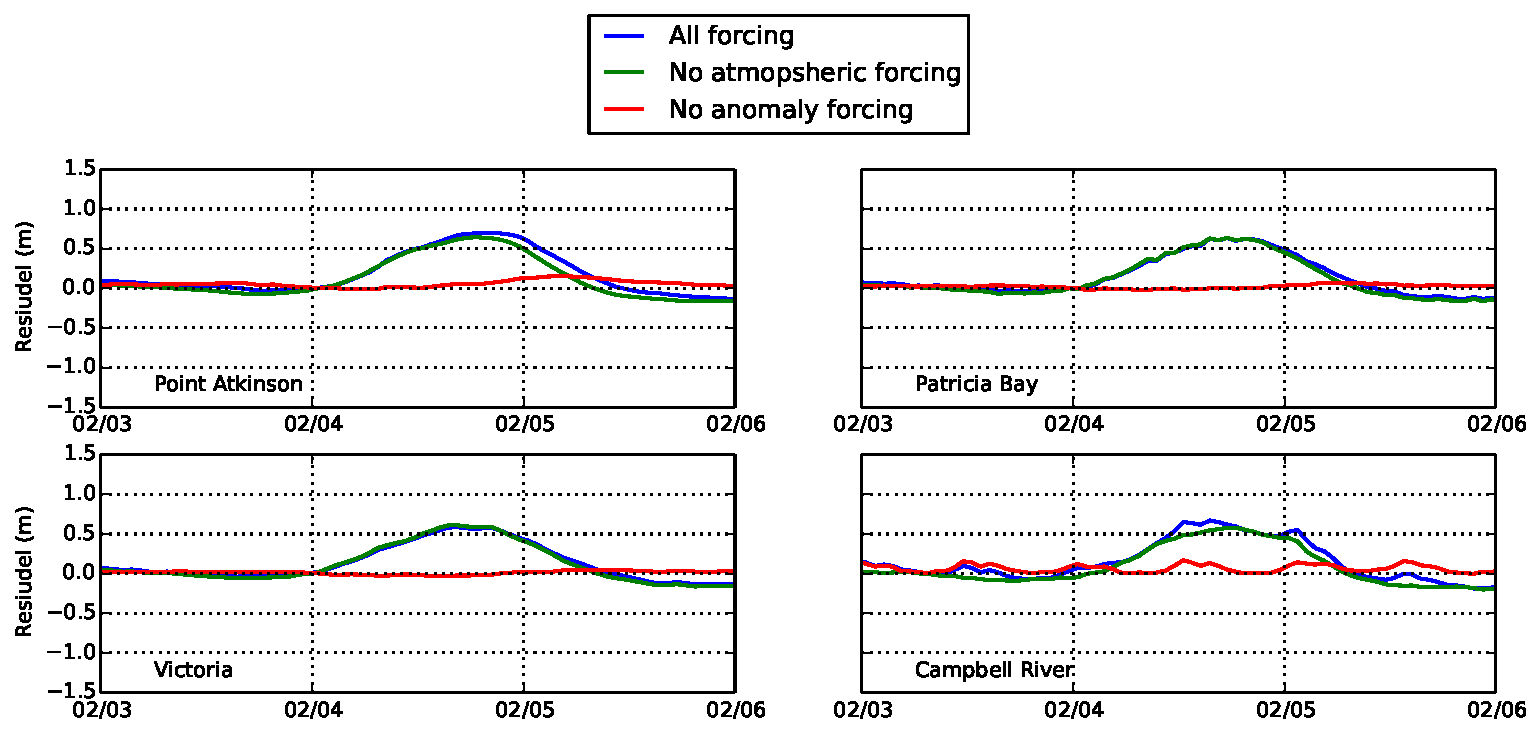
\includegraphics[scale=0.6]{Figures/feb2006_factors_bg.pdf}
\caption{Comparison of the modelled residual for three simulations: A simulation with all forcing (blue), a simulation without atmospheric forcing (green), and a simulation without the sea surface height anomaly (red). }
\label{fig:factors}
\end{figure}
%not sure about the colours, but different line styles is really hard to make out. 

Finally, an assessment of the importance of including tide-surge interactions is presented next. A simulation of the surge propagation without including any tidal forcing is compared with the modelled residual in Figure \ref{fig:tidesurge}. Recall, the modelled residual is defined as the difference between the sea surface height in a simulation with all forcing and a simulaltion with tides amd rivers only. A comparison between the modelled residual and a surge only run can determine the significance of the tide-surge interaction. This figure shows there is almost no difference between the simulations at all locations, rendering the tide-sure interaction negligible. In operational settings, running a surge only simulation and adding the predicted tides a posteriori could be more computationally efficient with only a small decrease in the accuracy of the prediction. 
% I'm not sure if removing a background state is really appropriate here. There could be some differences in the background states because of the tides(ie where fresh water moves to, etc). I also think it is more appropriate to use the atmospheric pressure to remove the background state...

%Finally, an assessment of the importance of including tide-surge interactions is presented next. A simulation of the surge propagation without including any tidal forcing is compared with the modelled residual in Figure \ref{fig:tidesurge}. Recall, the modelled residual is defined as the difference between the sea surface height in a simulation with all forcing and a simulaltion with tides amd rivers only. A comparison between the modelled residual and a surge only run can determine the significance of the tide-surge interaction. The most significant differences occur at Point Atkinson where the maximum modelled residual is 7 cm higher than the maximum of the surge only case.  In contrast, the tide-surge interaction at Victoria is hardly noticeable. Indeed, a spatial map of the modelled residual and surge only differences (not shown here) indicate that the tide-surge interaction is more pronounced after the San Juan and Gulf Islands. The passages between these islands are known for vigorous tidal mixing, which may have an effect on the surge propagation. However, the effect is a relatively small underestimate of the surge elevation and no changes to the timing of the surge. So, in operational settings, running a surge only simulation and adding the predicted tides a posteriori could be more computationally efficient with only a small decrease in the accuracy of the prediction. 

\begin{figure}
\centering
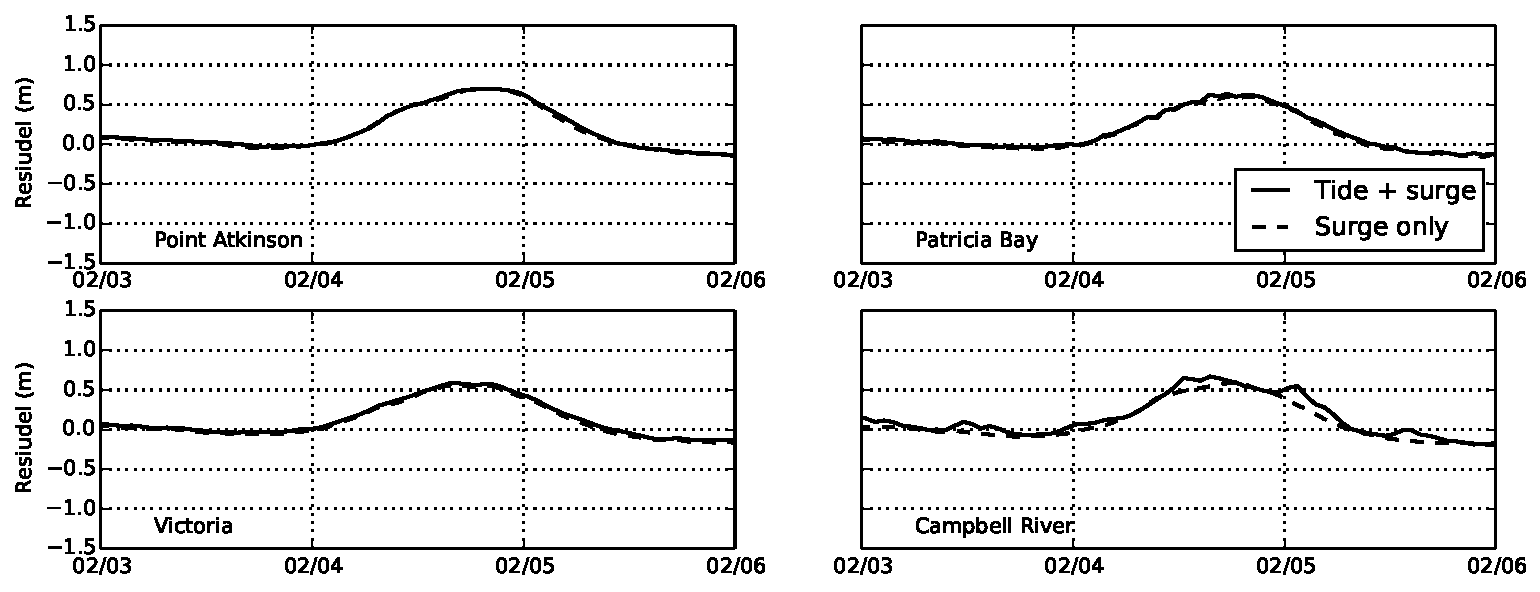
\includegraphics[scale=0.6]{Figures/feb2006_tidesurge_bg.pdf}
\caption{Modelled residuals (solid) compared a simulation of the surge propagation without tidal forcing (dashed).}
\label{fig:tidesurge}
\end{figure}

\subsection{Spatial Extent of Surge: Dec 15, 2006}
On Dec 15, 2006, a major storm with wind gusts over 120 km/hr caused significant damage to many coastal communities on the Pacific Northwest. Although the storm was very strong and the observed residual at Point Atkinson reached 84 cm, this event did not coincide with high tide and so no siginificant or reported flooding occurred in the Vancouver area\citep{forseth2006adaptation}. This event has been used to examine the propgation of the surge throughout the domain. First, an assessment of the accuracy of the hindcast is provided. 

Point Atkinson observed a maximum surge amplitude of 84 cm, which is approximately 20 cm higer than the model result, however the timing of the surge agrees almost exactly. The best agreement occurs at Victoria where the observed surge was 62 cm and the model returned 54 cm. At all of the locations, the model predicted the maximum surge to occur within 3.5 hours of the observed surge. Typically, the modelled surge was too early, in contrast to the later predictions in the Feb, 4 2006 case. Errors in the modelled water level at the time of maximum surge were of the same order as the errors in the surge amplitude.  

The evolution and spatial distribution of the surge is highlighted in Figure \ref{fig:spatial} where the modelled residual is plotted every two hours beginning on Dec 14 at 18:30. The surge enters the system from the Strait of Juna de Fuca and Johnstone Strait, peaking between Dec 15 at 6:30 and Dec 15 at 10:30 and then begins to subside throughout the entire domain. Notably, the Strait of Georgia experiences the largest surge values, upwards of 70 cm, whereas the Juan de Fuca region experiences a maximum surge around 55 cm. Additionally, the coastal areas on the mainland side of the Strait of Georgia experience slightly higher surges than the Vancouver Island side, likley due to the southerly wind in the atmosheric model pushing water against the mainland coast.  

\begin{figure}
\centering
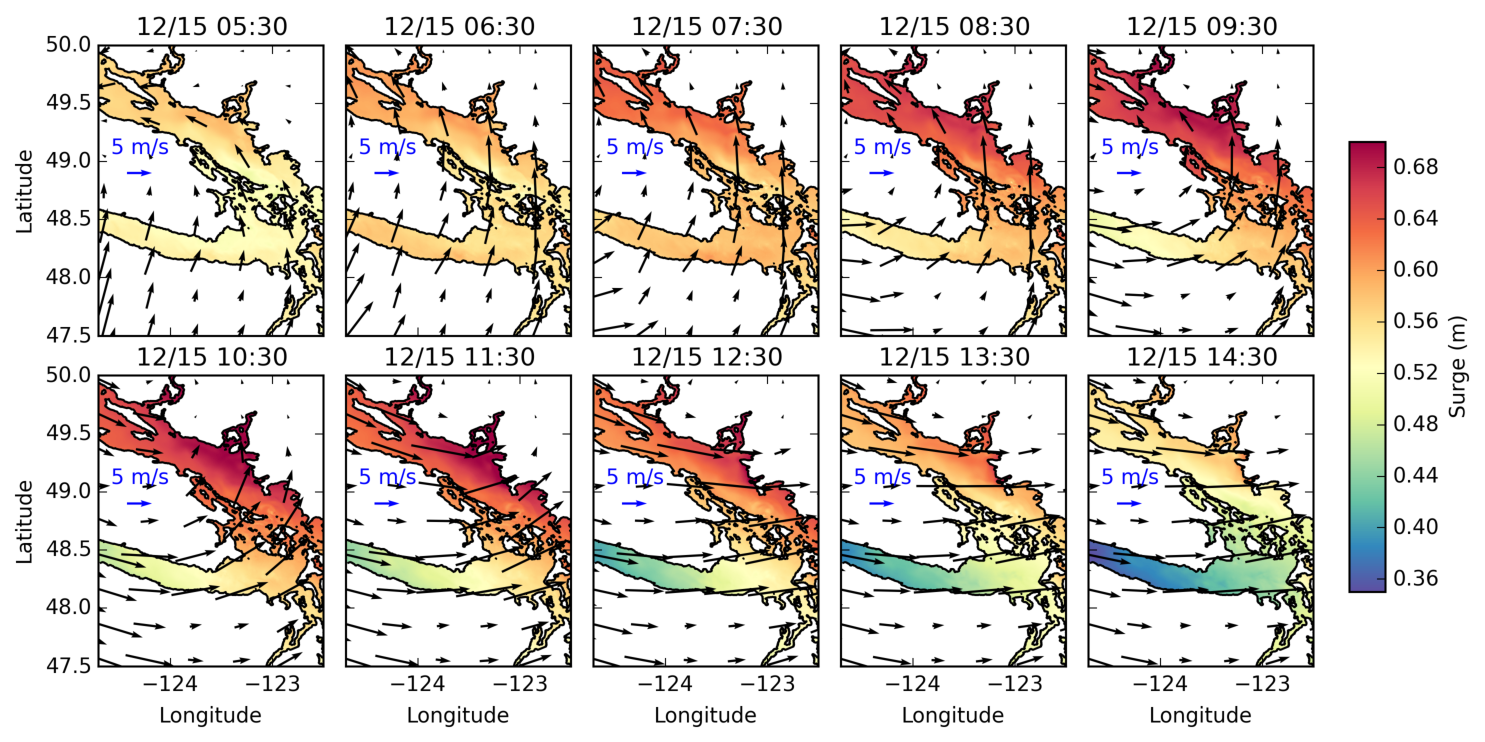
\includegraphics[scale=0.6]{Figures/dec2006_spatial.pdf}
\caption{Propagation of the storm surge on Dec 14/15 2006. Modelled residual every 2 hours starting on Dec 14 at 18:30. Time advances from top left to bottom right. Note that the images are oriented with the numerical grid which is rotated $29^{\circ}$ counter-clockwise of North. }
\label{fig:spatial}
\end{figure}

\subsection{Strong Wind Event: Nov 18, 2009}

\subsection{High Resolution Atmospheric Forcing: Dec 17, 2012}

\subsection{Statisitics}
%I think Hal Ritchie's talk with the storm surges had some stats presented. Look this up...

\section{Discussion}\label{sec:diss}
%future directions: running real time, biology and chemistry, model improvements?
%comments on wetting and drying (maybe most imporant in shallow regions)

\section{Acknowledgements}\label{sec:ack}
We would like to thank Michael Foreman, Diane Masson, and Luc Fillion for providing data used in model set up and evaluation. This project is funded by the Marine Environmental Observation Prediction and Response Network (MEOPAR), a Network of Centres of Excellence of Canada.  
%I'm likely missing a lot more (Keith, Youyu, Vasily, JP, Rich, Mark). Not sure about authorship but something to think about for later....

\bibliographystyle{chicago}
\bibliography{ref}

\end{document}

